The process for bootstrap calibrating the WWLLN stations and how the energy is calculated is described in \citet{Hutchins2012}.
This section walks through the code used in the processing along with the decisions behind various checks and adjustments made in the processing.

\section{Code Summary}

There are 8 main sections to the bootstrap processing:

\begin{itemize}
	\item{Process R-files into AP-files}
	\item{Calculate LWPC attenuation coefficients for each stroke-station pair}
	\item{Bootstrap calibrate the network}
	\item{Calculate stroke energy using LWPC and calibration}
	\item{Iterative re-calibrate the network}
	\item{Final energy calculation}
	\item{Run Relative Detection Efficiency Model (Chaper~\ref{thesis:chapter:efficiency})}
	\item{Move files to storage locations}
\end{itemize}

This processing requires several files, locations given relative to mlhutch@flash5.ess.washington.edu.

\begin{itemize}
	\item{\textbf{$\sim$/Process/relocate-B31Jan2013.x86-64} -- James Brundell's relocate program used to process R-files into AP-files, this version compiled for Linux 64-bit systems}
	\item{\textbf{stations.dat} -- list of current WWLLN stations, copied over from flash4 at the start every processing run.}
	\item{\textbf{lwpcv21} -- directory containing a working compiled version of the LWPC code.
		Used in generating new lookup tables as stations are added, a parallelized matlab implementation is discussed below.
		Provided as a sub-module of the Bootstrap directory.}
	\item{\textbf{$\sim$/matlab/Bootstrap/} -- directory containing the necessary matlab files, available as a git directory (see Appendix~\ref{thesis:appendix:code}).}
	\item{\textbf{Detection Efficiency} -- The code for modeling the network relative detection efficiency.
		Provided as a sub-module of the Bootstrap directory.}
	\item{\textbf{$\sim$/matlab/functions/} -- directory of necessary matlab functions used by the Bootstrap code files, also available as a git directory (see Appendix~\ref{thesis:appendix:code}).}
\end{itemize}

\section{LWPC}

The Long Wave Propagation Capability code is a codebase developed by \citet{Ferguson1998} that is used to calculated the electric field at a given location for a VLF transmitter at another location.
For the WWLLN energy processing it is used to estimate the attenuation between a stroke (treated as a transmitter) and a station.
The original LWPC code has been altered in two ways: first the Windows-compiler specific code has been replaced with GCC compilable code, second all warning have been removed to produce output of a constant shape (for reading into MATLAB).
All edits in the source code have been marked by my initials of MH.

\subsection{Compiling}

To recompile LWPC two bash scripts need to be run.
The first is \textbf{BuildData.cmd}, BuildData recompiles the data files that contain the surface parameters such as ground conductivity and coastlines.
The second step is to run \textbf{buildlwpc.cmd}, this should compile the program and result in an executable called LWPC.
To test a successful compile run the script \textbf{run\_bench.cmd}, if it runs successfully it is compiled, if not consult the \textbf{Readme - Unix.txt} file that has some common troubleshooting steps.

The last step in setting up LWPC is to set the \textbf{lwpcDAT.loc} file to point towards the \textbf{data} folder.

\subsection{Running}

LWPC is run from the command line with the structure:

\begin{verbatim}
./LWPC test1.inp
\end{verbatim}

Where \textbf{test1.inp} is formatted as per the structure in \textbf{User\_manual.pdf}.
The matlab implemtations discussed below automatically generate formatted input files.

The result of running LWPC is an output file the specifies the electric field at various distance along the path from the transmitter to receiver.
It is also capable of outputting plots, azimuthal dependence, and many other features not utilized in this research.

\subsection{Matlab Function}

A matlab implementation of LWPC is available as a git repository (see Appendix~\ref{thesis:appendix:code}).
This implantation allows for LWPC to called in matlab with:

\begin{verbatim}
LWPCpar(freq,lat,long,time,stat_lat,stat_long,model)
\end{verbatim}

Where freq is the transmitter frequency, lat/long is the transmitter location, time is the date and time, stat\_lat/stat\_long are the receiver locations, and model is the ionospheric model used.
If model is set to ``time'' then day and night is considered in the calculation, if it is set to ``day'' or ``night'' an all day or all night ionosphere will be used.

LWPCpar as the advantage of being runnable within matlab parallelized loops (parfor).
While LWPC itself cannot be run in parallel, this method simply copies the LWPC directory to allow each matlab instance it's own copy.

\section{Lookup Tables}

While LWPC can be parallelized it is still too slow to run faster than realtime for WWLLN processing.
As a result two sets of lookup tables are generated for each station with the pre-calculated LWPC electric field values.

The lookup tables are part of the main Bootstrap directory under the names \textbf{lookup\_day.dat} and \textbf{lookup\_night.dat}.
Each of these files are tab-delimited text with the format given in Table~\ref{bootstrap:table:lookup}.
The tables list the electric field measured the the station given a 100~kW transmitter in each grid point on the globe.
The latest lookup tables are at a resolution of $2^\circ$.

\begin{table}[h!]
\begin{center}
\begin{tabular}{|p{1.5in}|p{1.75in}|p{1.75in}|p{1in}|}
\hline
\rule{0pt}{3ex}
Station Name	&Station North Latitude	&	Station East Longitude & \\ 
\hline
\rule{0pt}{3ex}
E-field at (-179,89)	& E-field at (-177,89) &	E-field at (-175,89) & \dots \\ 
\hline
\rule{0pt}{3ex}
E-field at (-179,87)	& E-field at (-177,87) &	E-field at (-175,87) & \dots \\ 
\hline
\rule{0pt}{3ex}
E-field at (-179,85)	& E-field at (-177,85) &	E-field at (-175,85) & \dots \\ 
\hline
\rule{0pt}{3ex}
\dots	& \dots &	\dots & \dots \\ 
\hline
\end{tabular}
\end{center}
\caption{Format for \textbf{lookup\_day.dat} and \textbf{lookup\_night.dat} data files for a resolution of $2^\circ$.}
\label{bootstrap:table:lookup}
\end{table}

An example of a lookup table for the all day ionosphere for Dunedin station is shown in Figure~\ref{bootstrap:fig:lookup}.

\begin{figure}[ht!]
   \centering
   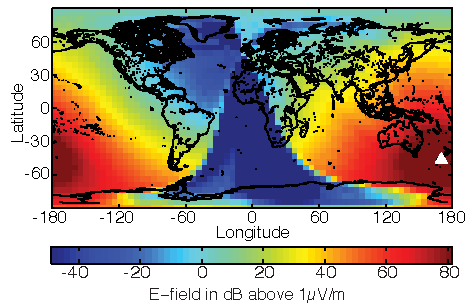
\includegraphics[scale=1]{Energy/Figures/PPS_Lookup.pdf} 
   \caption{Lookup table for an all day ionosphere for Dunedin station.}
   \label{bootstrap:fig:lookup}
\end{figure}

\subsection{Generation}

The LWPC lookup tables are generated automatically with the matlab script {\bf $\sim$/Bootstrap/\\Lookup\_automation.m} that is called at the start of the daily energy processing.
The script checks the current number of stations in the \textbf{.dat} files and compares it to the most recent \textbf{stations.dat} file.
If there are a new entries in the \textbf{stations.dat} then the script proceeds to make the lookup tables.

The automatic script calculates the electric field at every grid point for 11 frequencies ranging from 8~kHz to 18~kHz, and averages them together to add to the \textbf{.dat} files.

The same script can be run for specific stations with the \textbf{$\sim$/matlab/lwpcpar/lwpc\_generate.m} script.

Tables generated with either script can be validated with the \textbf{$\sim$/matlab/Bootstrap/\\lookup\_validation.m} scipt.
This script checks each grid point to ensure there is a real number there, sometimes LWPC generates errors for very specific locations.
If there is no valid electric field value at that spot it is reprocessed by offsetting the transmitter by a fraction of a degree.

\section{Matlab Code}

The main matlab script to run the entire energy calculation process is {\bf Boostrap\_automation.m}.
This script:
\begin{enumerate}
\item{Defines the dates to run (in case past days need to be rerun)}
\item{Sets the system path parameters from {\bf data\_path.m}}
\item{Updates stations.dat and the lookup tables {\bf Lookup\_automation.m}.}
\item{Generate the current AP-file with {\bf generate\_ap.m}}
\item{Calculate the energies and station calibrations using {\bf wwlln\_energy.m}}
\item{Generates the relative detection efficiency map with {\bf de\_mapper.m}}
\item{Saves and archives all of the resulting data files}
\end{enumerate}

In order to rerun lost days the only change necessary for Bootstrap\_automation is to change the rundate from:

\begin{verbatim}
		RUNDATE = floor(now - 1);
\end{verbatim}

to the day (or dates) that need to be rerun.
The LIVE variable and second part of the if clause is for rerunning \emph{previously processed} data.
If LIVE is set to false then the script runs and stores in an alternative directory with a copy of the resulting calibration file.
For the case of restarting the script on the same day it failed to run, no changes need to be made.

\subsection{data\_path.m}

It is important to correctly set up the {\bf data\_path.m} script. 
Aside from the storage paths, it is important to set how the script should obtain the stations.dat and R-files from flash4.
The transfer type can either be cp if the computer has flash4 network mounted, or scp if passwordless scp is setup.
The r\_path\_flat variable determines whether the R-files are stored in one directory or with a hierarchal structure (e.g. /wd2/Rfiles/R2013/R201304/R201304*).

Additionally the location of the bootstrap processing folder itself as well as the TOGA relocate script.

\subsection{Lookup\_automation.m}

The {\bf Lookup\_automation.m} script compares the current number of entries in the lookup\_day.dat data file and compares it to the latest stations.dat file.
If stations.dat has new entries, then the script generates the corresponding LWPC lookup tables for those new stations.

Using the current lookup spatial resolution LWPCpar is called for each grid point at 11 frequencies (8 -- 11~kHz) for both day and night.
The 11 values in each grid point (in dB) are averaged together and added to the existing lookup data files.

This code takes about twelve hours to run using a single core due to calling the LWPC code.
The LWPCpar.m function is set up to run in parallel (it copies the LWPC code to new locations), however the {\bf Lookup\_automation.m} script has not be parallelized.

\subsection{generate\_ap.m}

{\bf generate\_ap.m} copies over the R-files to the TOGA relocate folder and processes them with the -e flag.
This generate the normal WWLLN A-file structure, with the addition of the participating stations and their RMS electric field values at the end of each line.
The RMS electric field (as mentioned elsewhere) is in the uncalibrated sound card units, where the calibration is the main part of the wwlln\_energy.m code.
The script ends with moving the new AP file and R-files to their storage locations.

\subsection{wwlln\_energy.m}

The {\bf wwlln\_energy.m} function runs the subfunctions described below in order to calculate the stroke energies.
Unless it is set otherwise (which it should be), the script sets the default master station to use to be Scott Base with the most recent calibration.
The master station is one with a known calibration that is used to bootstrap the calibrations for the rest of the network.
One future upgrade to the code would be the ability to include multiple master stations and combine their results for a better system-wide calibration.

The script also generates and saves two sets of station ratios.
The first is the station conversion file, the values in this file give how to convert the sound card units at the master station to the sound card units at the other stations.
It is saved in the case that the master calibration requires a retroactive change.
The calibration file gives the values to convert from individual station sound card units to RMS electric-field values.
The station calibration incorporates both the actual station calibration and any environmental changes near the station.

{\bf apply\_lwpc.m} applies the LWPC lookup tables to each sound card value in each stroke-station pair.
The day and night lookup table values are weighted by the percent of the path in daytime and nighttime.
There is also a distance range restriction, where only stroke-station values between 1 and 8~Mm are calculated, otherwise they are given a value of zero.

{\bf cross\_calibration.m} finds all strokes common to each pair of stations, and uses them to create a conversion ratio between every pair of stations.
Only if the two stations have common strokes in all day paths and are within the same 1 -- 8~Mm distance restriction.
The median value of every common stroke value is used as the resulting station-pair conversion ratios.

{\bf bootstrap.m} solves the connected graph of station-pair conversions to find the valid calibration paths from the master station to every other possible station.
There are two ways for a station to be added as a well calibrated station.
First it can have common strokes between itself and the master station, this would result in a single hop conversion.
The second way is to be calibrated off of one of the previously calibrated stations.
In this case a secondary (or tertiary etc.) calibration is validated by comparing it's direct conversion with a conversion using it as an intermediary.
So to test if the calibration of A to B is valid, B is used in the A to B to C calibration.
If the ABC calibration matches the direct AC calibration to within 75\% then B is considered well calibrated.
This bootstrapping is conducted for 5 hops, so any converted station is at most 4 intermediary stations away from the master station.

{\bf conversion\_check.m} takes the resulting calibration paths from bootstrap.m and performs the bootstrap calibration using the initial calibration of the master station and the conversion ratios of cross\_calibration.m.
It also requires that the master station is included in the case where it becomes excluded in the bootstrap.m subfunction.

To prevent sudden changes in gain or wildly varying station from being included {\bf conversion\_mean.m} checks the new calibration values against the previous 7 days of calibrations.
If the new calibration is not drastically different then the average of the previous 7 days of calibration values is used as the calibration value, otherwise it is excluded.
A station is deemed unstable if one of the past seven days is either larger or smaller than the median by a factor of 10 (normalized by Scott Base, Dunedin, and Seattle).

{\bf stroke\_energy.m}
Applies the calibration
Median
MAd

{\bf energy\_iterate.m}
Runs stroke\_energy 5 times
Uses strokes are ground truth to recalibrate
converges

Save and store data, calibrations, and conversions

\section{Relative Detection Efficiency Code}

\subsection{Point to Paper}

\subsection{Code Summary}

\subsection{Code Description and Location}

\subsection{Output Interpretation}

\subsection{Matlab Code}